\subsection{Consistency in the case of free electrons}
\begin{figure}
    \centering
    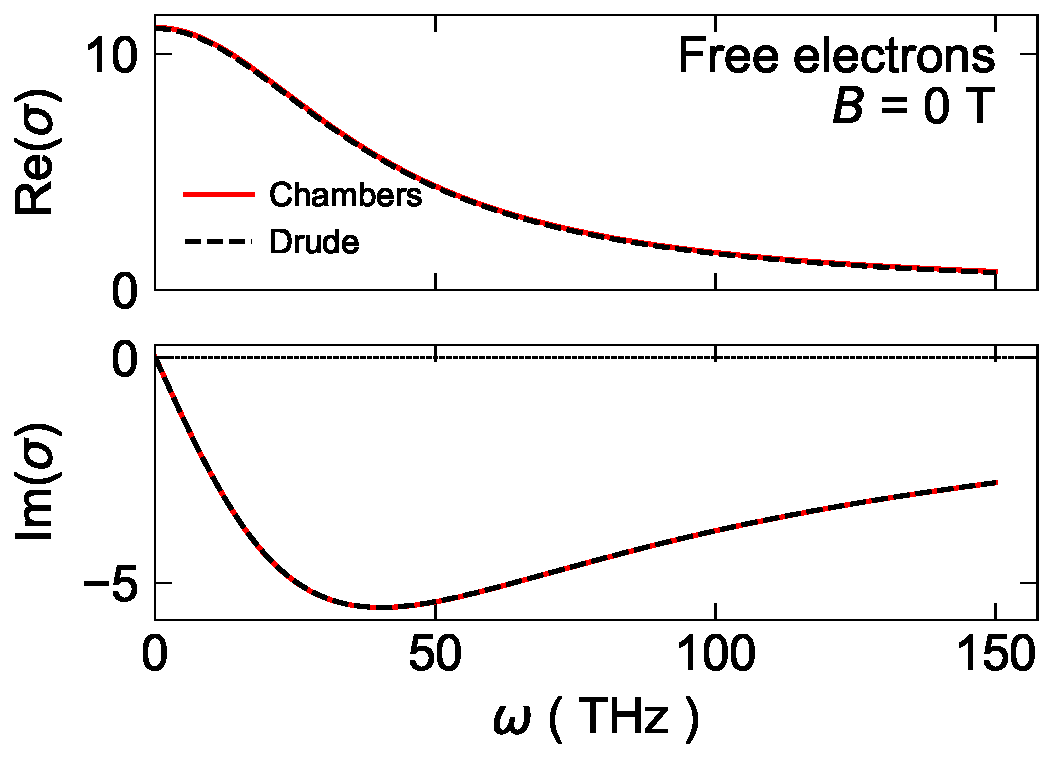
\includegraphics[width=0.7\textwidth]{figures/free_electrons}
    \caption{Agreement of the Drude and Chambers models for free electrons.}
    \label{fig:free_electrons}
\end{figure}

To make sure our new model makes sense, we need some form of validation. Since the Drude model works
well for non-anisotropic materials, having ``free'' electrons, the Chambers model should produce
results that are consistent with the Drude model in this case. We showed that this is mathematically
true (\textcolor{red}{TODO: appendix}).

After equipping the numerical package with the ability to cacluate optical conductivity, we compared
the output of our implementation of the Chambers model to the Drude model for free electrons. Figure
\ref{fig:free_electrons} shows how the two models agree for free electrons. We used this case for
validating our implementation of the Chambers model.